\section{Teilaufgabe 19}
\begin{aufgabe}
    Skizzieren Sie das Bode-Diagramm des offenen Regelkreises für $T_i > 
    \tau_g$ und $T_i < \tau_g$.
\end{aufgabe}
\[ L(s) = K_p \cdot \left(1 + \frac{1}{T_i \cdot s}\right) 
    \cdot \frac{K_g}{\tau \cdot s + 1}
\]
\[ T_i > \tau_g \]
\begin{figure}[h!]
    \centering
    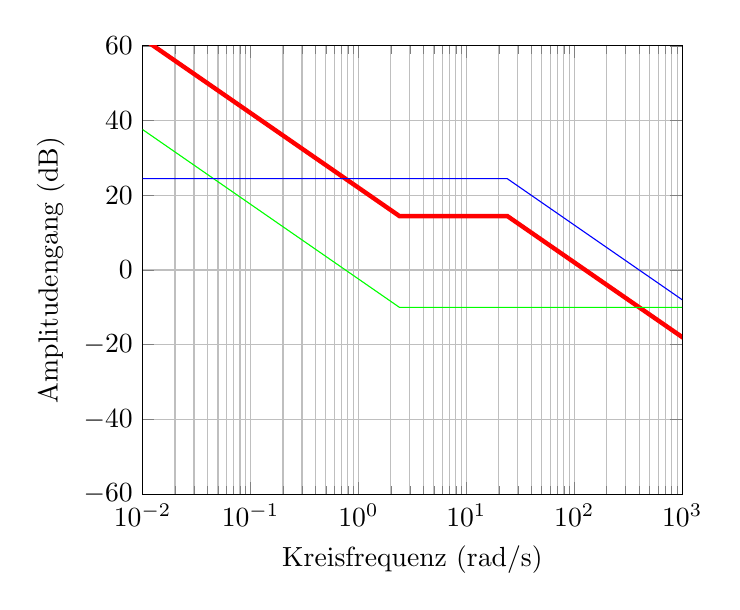
\begin{tikzpicture}[scale=1]
        \begin{semilogxaxis}
            [xmin=1e-2, 
                xmax=1e3, 
                ymin=-60, 
                ymax=60, 
                ytick={-60, -40, ..., 60}, 
                xlabel=Kreisfrequenz (rad/s),
                ylabel=Amplitudengang (dB),
                grid=both]
            \addplot[mark=none, color=red, ultra thick] coordinates 
                {(0.002398,74.420) 
                (2.398,14.430) 
                (23.98,14.430) 
                (2398,-25.57)};
            \addplot[mark=none, color=green] coordinates 
                {(0.002398,50.000) 
                (2.398,-10.000) 
                (2398,-10.000)};
            \addplot[mark=none, color=blue] coordinates 
                {(0.002398,24.430) 
                (23.98,24.430) 
                (2398,-15.57)};
        \end{semilogxaxis}
    \end{tikzpicture}
    \\
    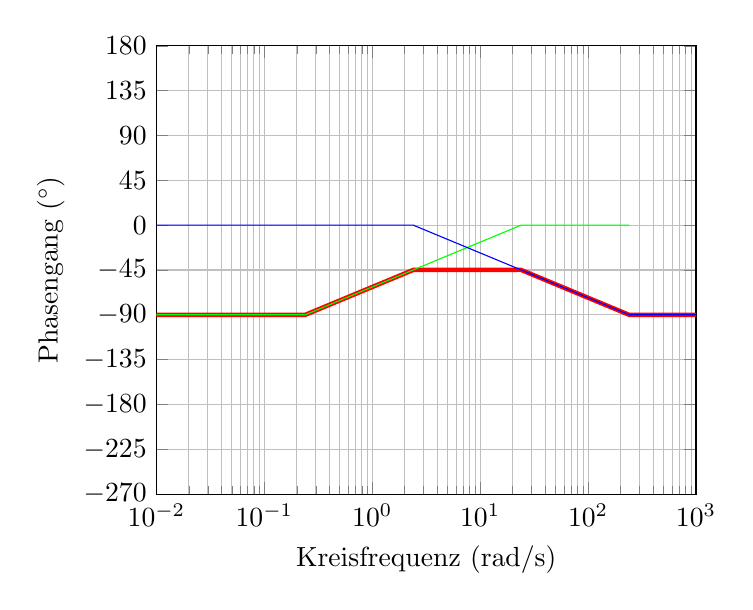
\begin{tikzpicture}[scale=1]
        \begin{semilogxaxis}
            [xmin=1e-2, 
                xmax=1e3, 
                ymin=-270, 
                ymax=180, 
                ytick={-270, -225, ..., 180}, 
                xlabel=Kreisfrequenz (rad/s),
                ylabel=Phasengang ($^\circ$),
                grid=both]
            \addplot[mark=none, color=red, ultra thick] coordinates 
                {(0.002398,-90) 
                (0.2398,-90) 
                (2.398,-45) 
                (23.98,-45) 
                (239.8,-90) 
                (2398,-90)};
            \addplot[mark=none, color=green] coordinates 
                {(0.002398,-90) 
                (0.2398,-90) 
                (23.98,0) 
                (239.8,0)};
            \addplot[mark=none, color=blue] coordinates 
                {(0.002398,0) 
                (2.398,0) 
                (239.8,-90) 
                (2398,-90)};
        \end{semilogxaxis}
    \end{tikzpicture}
\end{figure}
\\
\tikz{\draw[blue]               (0,0) -- (1,0);} $PT_1$ Strecke \\
\tikz{\draw[green]              (0,0) -- (1,0);} $PI$ Regler \\
\tikz{\draw[red, ultra thick]   (0,0) -- (1,0);} Regler und Strecke \\
\clearpage
\[ T_i < \tau_g \]
\begin{figure}[h!]
    \centering
    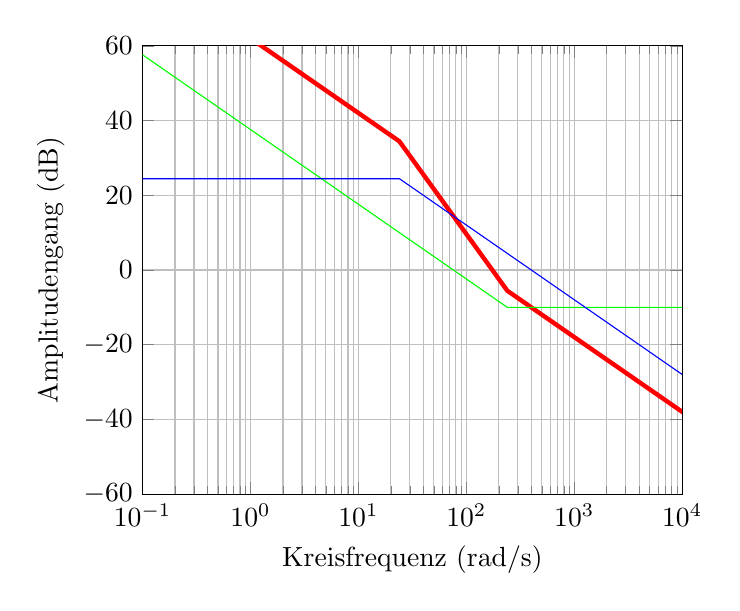
\begin{tikzpicture}[scale=1]
        \begin{semilogxaxis}
            [xmin=1e-1, 
                xmax=1e4, 
                ymin=-60, 
                ymax=60, 
                ytick={-60, -40, ..., 60}, 
                xlabel=Kreisfrequenz (rad/s),
                ylabel=Amplitudengang (dB),
                grid=both]
            \addplot[mark=none, color=red, ultra thick] coordinates 
                {(0.002398,114.420) 
                (23.98,34.430) 
                (239.8,-05.57) 
                (23980,-45.57)};
            \addplot[mark=none, color=green] coordinates 
                {(0.002398,90.000) 
                (239.8,-10.000) 
                (23980,-10.000)};
            \addplot[mark=none, color=blue] coordinates 
                {(0.002398,24.430) 
                (23.98,24.430) 
                (23980,-35.57)};
        \end{semilogxaxis}
    \end{tikzpicture}
    \\
    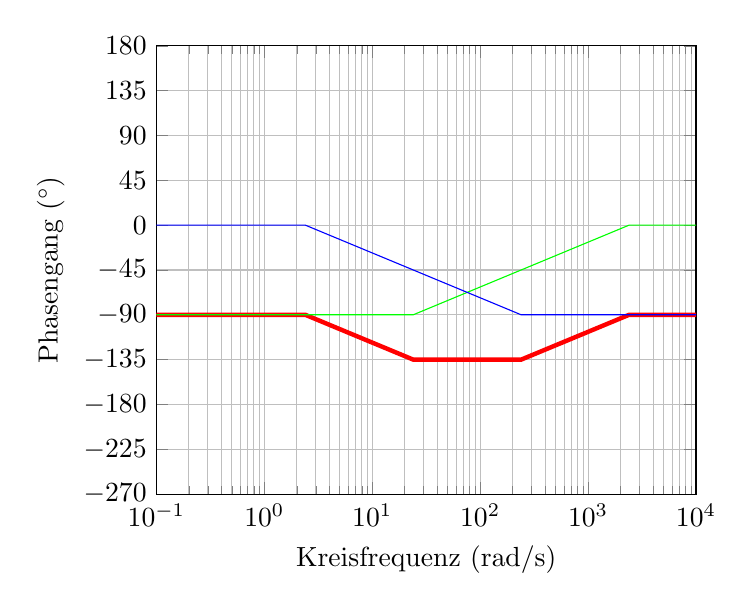
\begin{tikzpicture}[scale=1]
        \begin{semilogxaxis}
            [xmin=1e-1, 
                xmax=1e4, 
                ymin=-270, 
                ymax=180, 
                ytick={-270, -225, ..., 180}, 
                xlabel=Kreisfrequenz (rad/s),
                ylabel=Phasengang ($^\circ$),
                grid=both]
            \addplot[mark=none, color=red, ultra thick] coordinates 
                {(0.002398,-90) 
                (2.398,-90) 
                (23.98,-135) 
                (239.8,-135) 
                (2398,-90) 
                (23980,-90)};
            \addplot[mark=none, color=green] coordinates 
                {(0.002398,-90) 
                (23.98,-90) 
                (2398,0) 
                (23980,0)};
            \addplot[mark=none, color=blue] coordinates 
                {(0.002398,0) 
                (2.398,0) 
                (239.8,-90) 
                (23980,-90)};
        \end{semilogxaxis}
    \end{tikzpicture}
\end{figure}
\\
\tikz{\draw[blue]               (0,0) -- (1,0);} $PT_1$ Strecke \\
\tikz{\draw[green]              (0,0) -- (1,0);} $PI$ Regler \\
\tikz{\draw[red, ultra thick]   (0,0) -- (1,0);} Regler und Strecke \\
